
\documentclass[12pt]{article}
\usepackage[margin=0.8in]{geometry} % Adjust margins to save space
\usepackage{amssymb}
\usepackage{graphicx}
\renewcommand{\baselinestretch}{1.1} % Slightly reduce line spacing
\usepackage{amsfonts}
\usepackage{amsmath}
\usepackage{amsthm}
\usepackage{tikz}
\usepackage{float}

\usepackage[colorlinks]{hyperref}
\usepackage{color}

\usepackage[english]{babel}
\usepackage[T1]{fontenc}
\usepackage[utf8]{inputenc}
\usepackage{subcaption}
\usepackage{csquotes}
\usepackage[procnames]{listings}
\definecolor{keywords}{RGB}{255,0,90}
\definecolor{comments}{RGB}{0,0,113}
\definecolor{red}{RGB}{160,0,0}
\definecolor{green}{RGB}{0,150,0}
\graphicspath{ {./images/} }
\usepackage[backend=biber,style=numeric]{biblatex}
\addbibresource{mybib.bib}
\setlength\parindent{0pt}

\author{Logi Ingvarsson}

\begin{document}
\selectlanguage{English}

\begin{flushleft}
{\large{\bf{SM2501 - Project 3}} \hfill Lorenzo Lucchini, Logi Ingvarsson, Lu Liu}
\end{flushleft}
\hrule height 1pt
\bigskip

\section{Part 1}

\subsection*{Work Methodology}
In accordance with instructions in the literature, we initiated calculations of activation in all main muscle groups, beginning with an initial stiffness value of 10,000. The maximum stiffness for the first iteration was set to 90,000, with incremental steps of 10,000 for generating the static optimization (SO) elaboration. To determine the stiffness yielding the lowest muscle activation, we developed a Python script that computed the average activation across each muscle group and identified the SO activation file corresponding to the minimum summed activation.

Our analysis indicated that a stiffness value of 60,000 minimized muscle activation. Subsequently, we refined the stiffness range, iterating between 60,000 and 62,000 with a step size of 100. This process revealed 61,000 as the optimal stiffness. Further refinement was performed with a step size of 10, examining stiffness values from 60,950 to 61,050. As the optimal stiffness remained unchanged at 61,000, we performed an additional fine-tuning analysis using a step size of 1 within the range of 60,990 to 61,010, confirming that 61,000 consistently minimized activation. This stiffness value was therefore selected for subsequent phases of the assignment.

\subsection*{Stiffness}

\begin{figure}[H]
    \centering
    \begin{subfigure}[b]{0.42\textwidth} % Reduced width
        \centering
        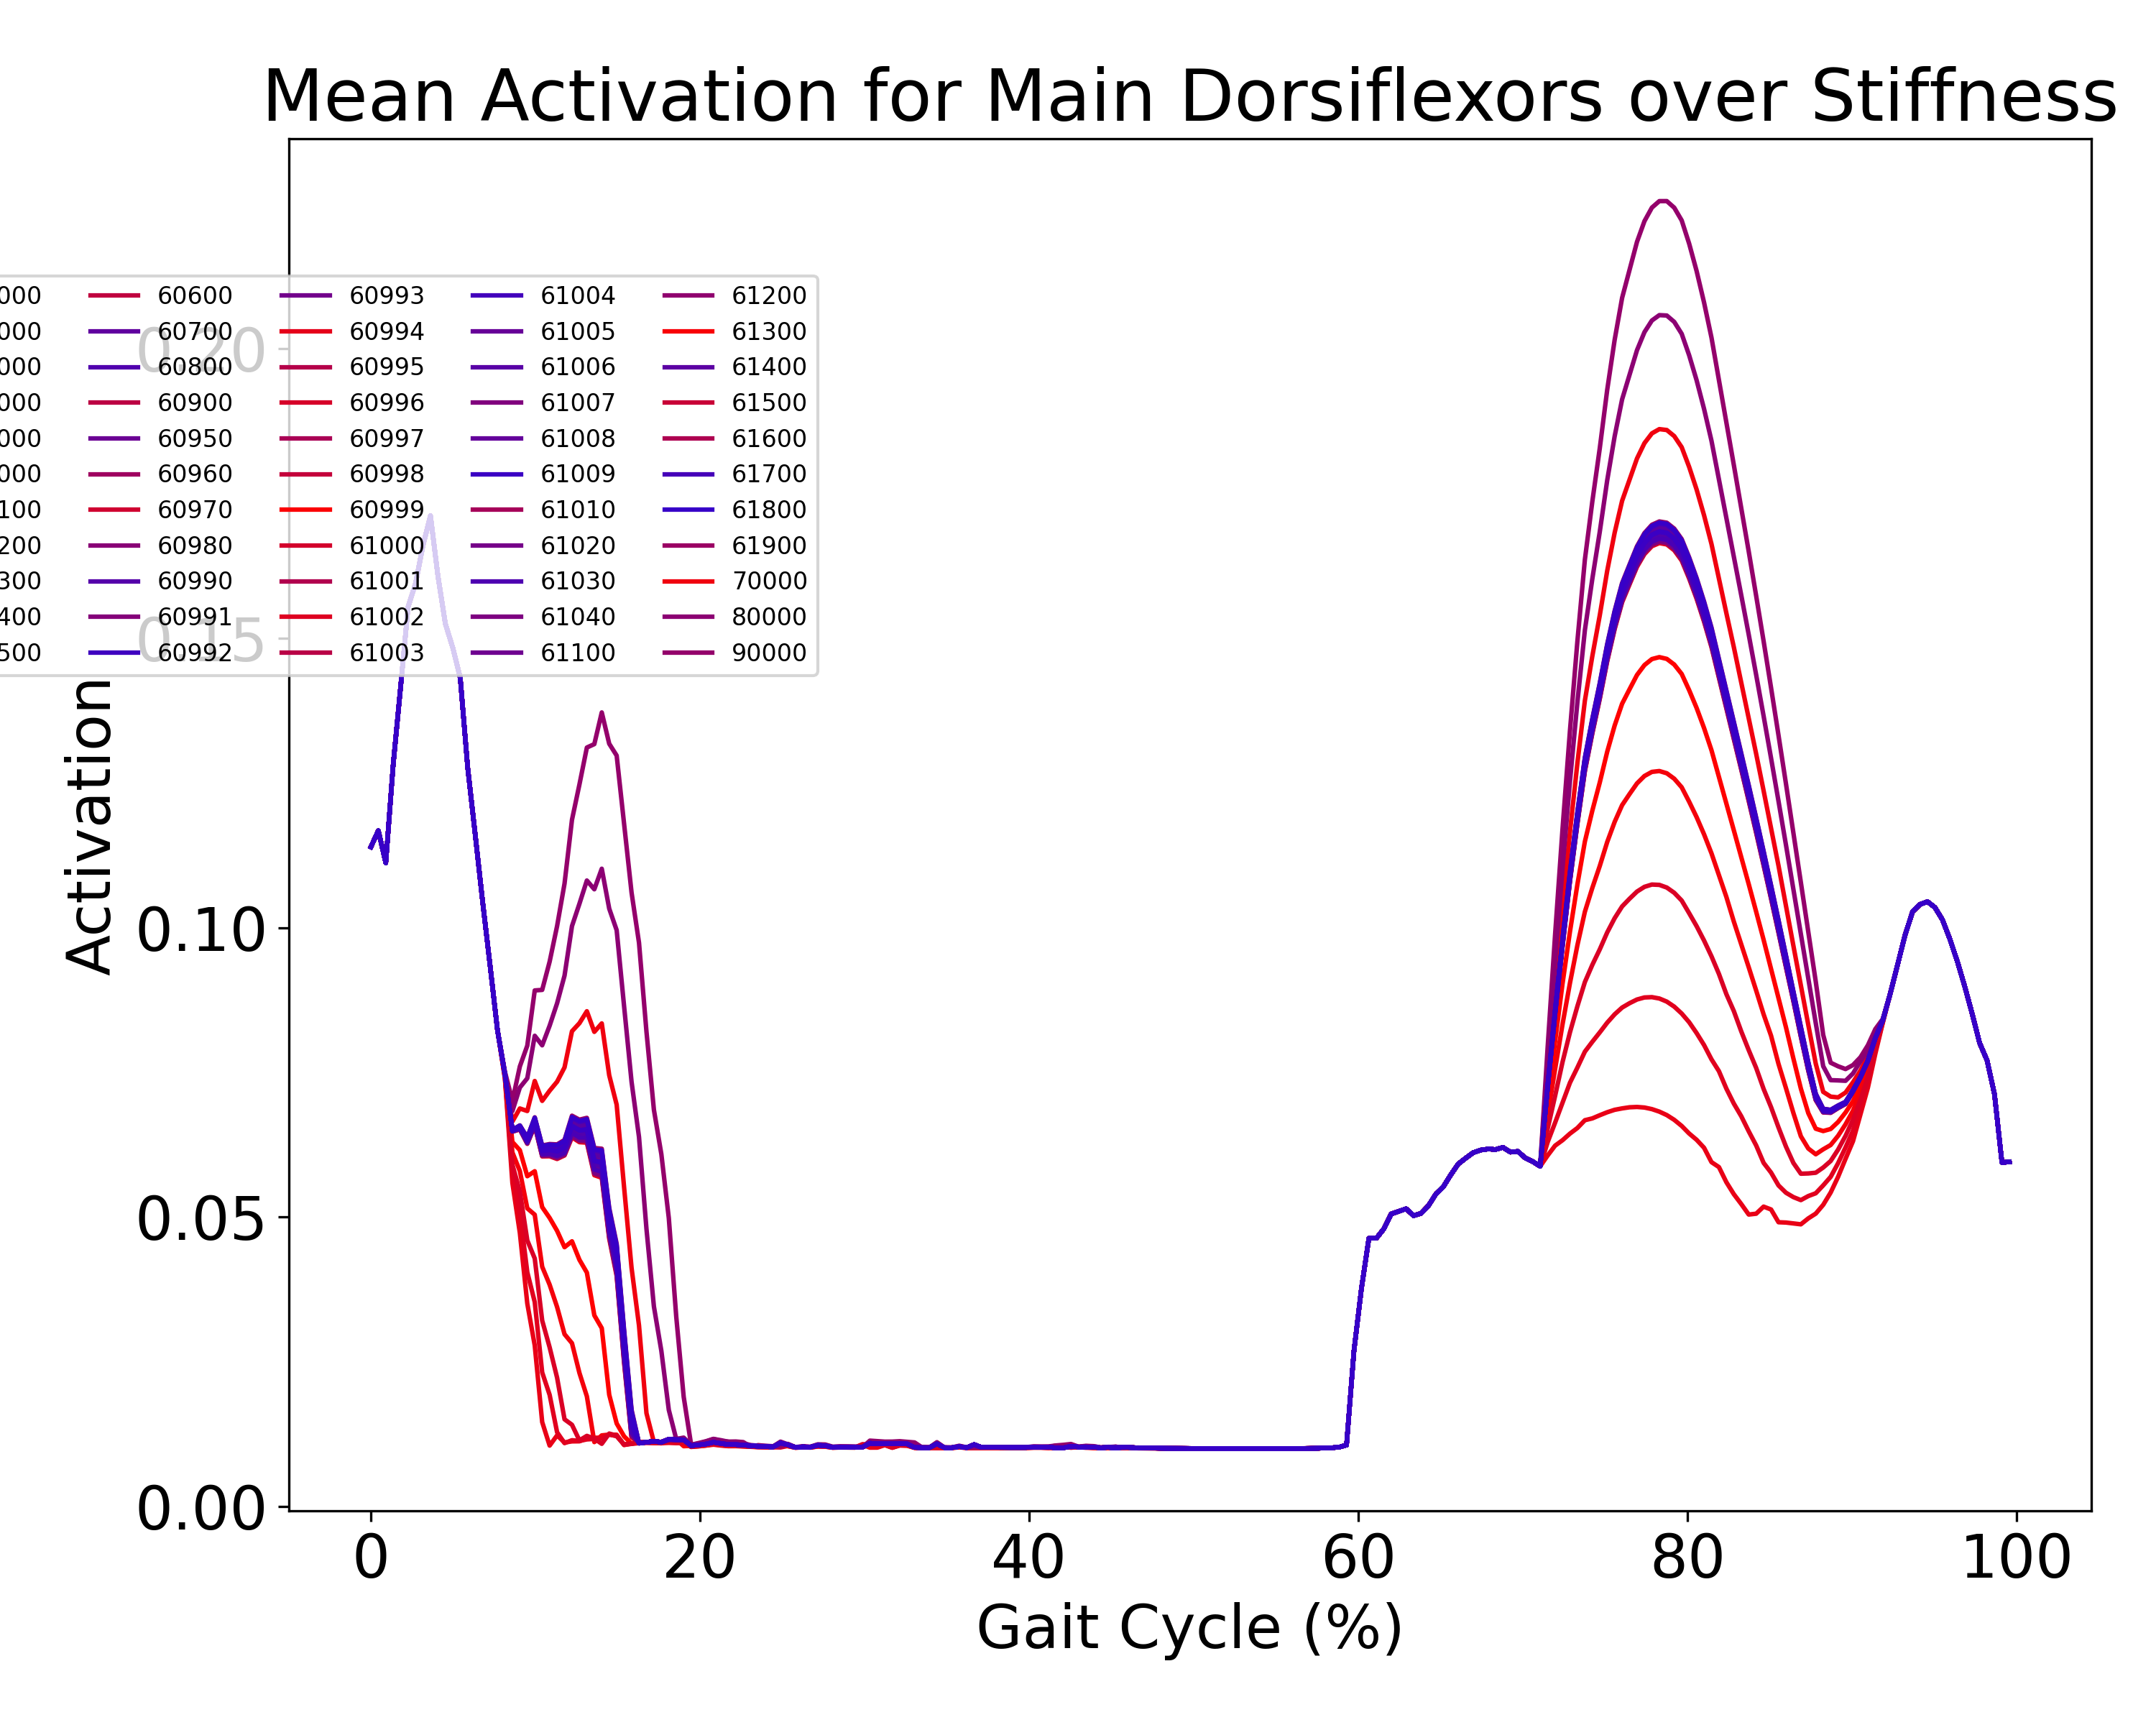
\includegraphics[width=\textwidth]{plots/stiffness/ActivationAcrossStiffness/TotalDorsiflexorsStiffness.png}
    \end{subfigure}
    \hfill
    \begin{subfigure}[b]{0.42\textwidth} % Reduced width
        \centering
        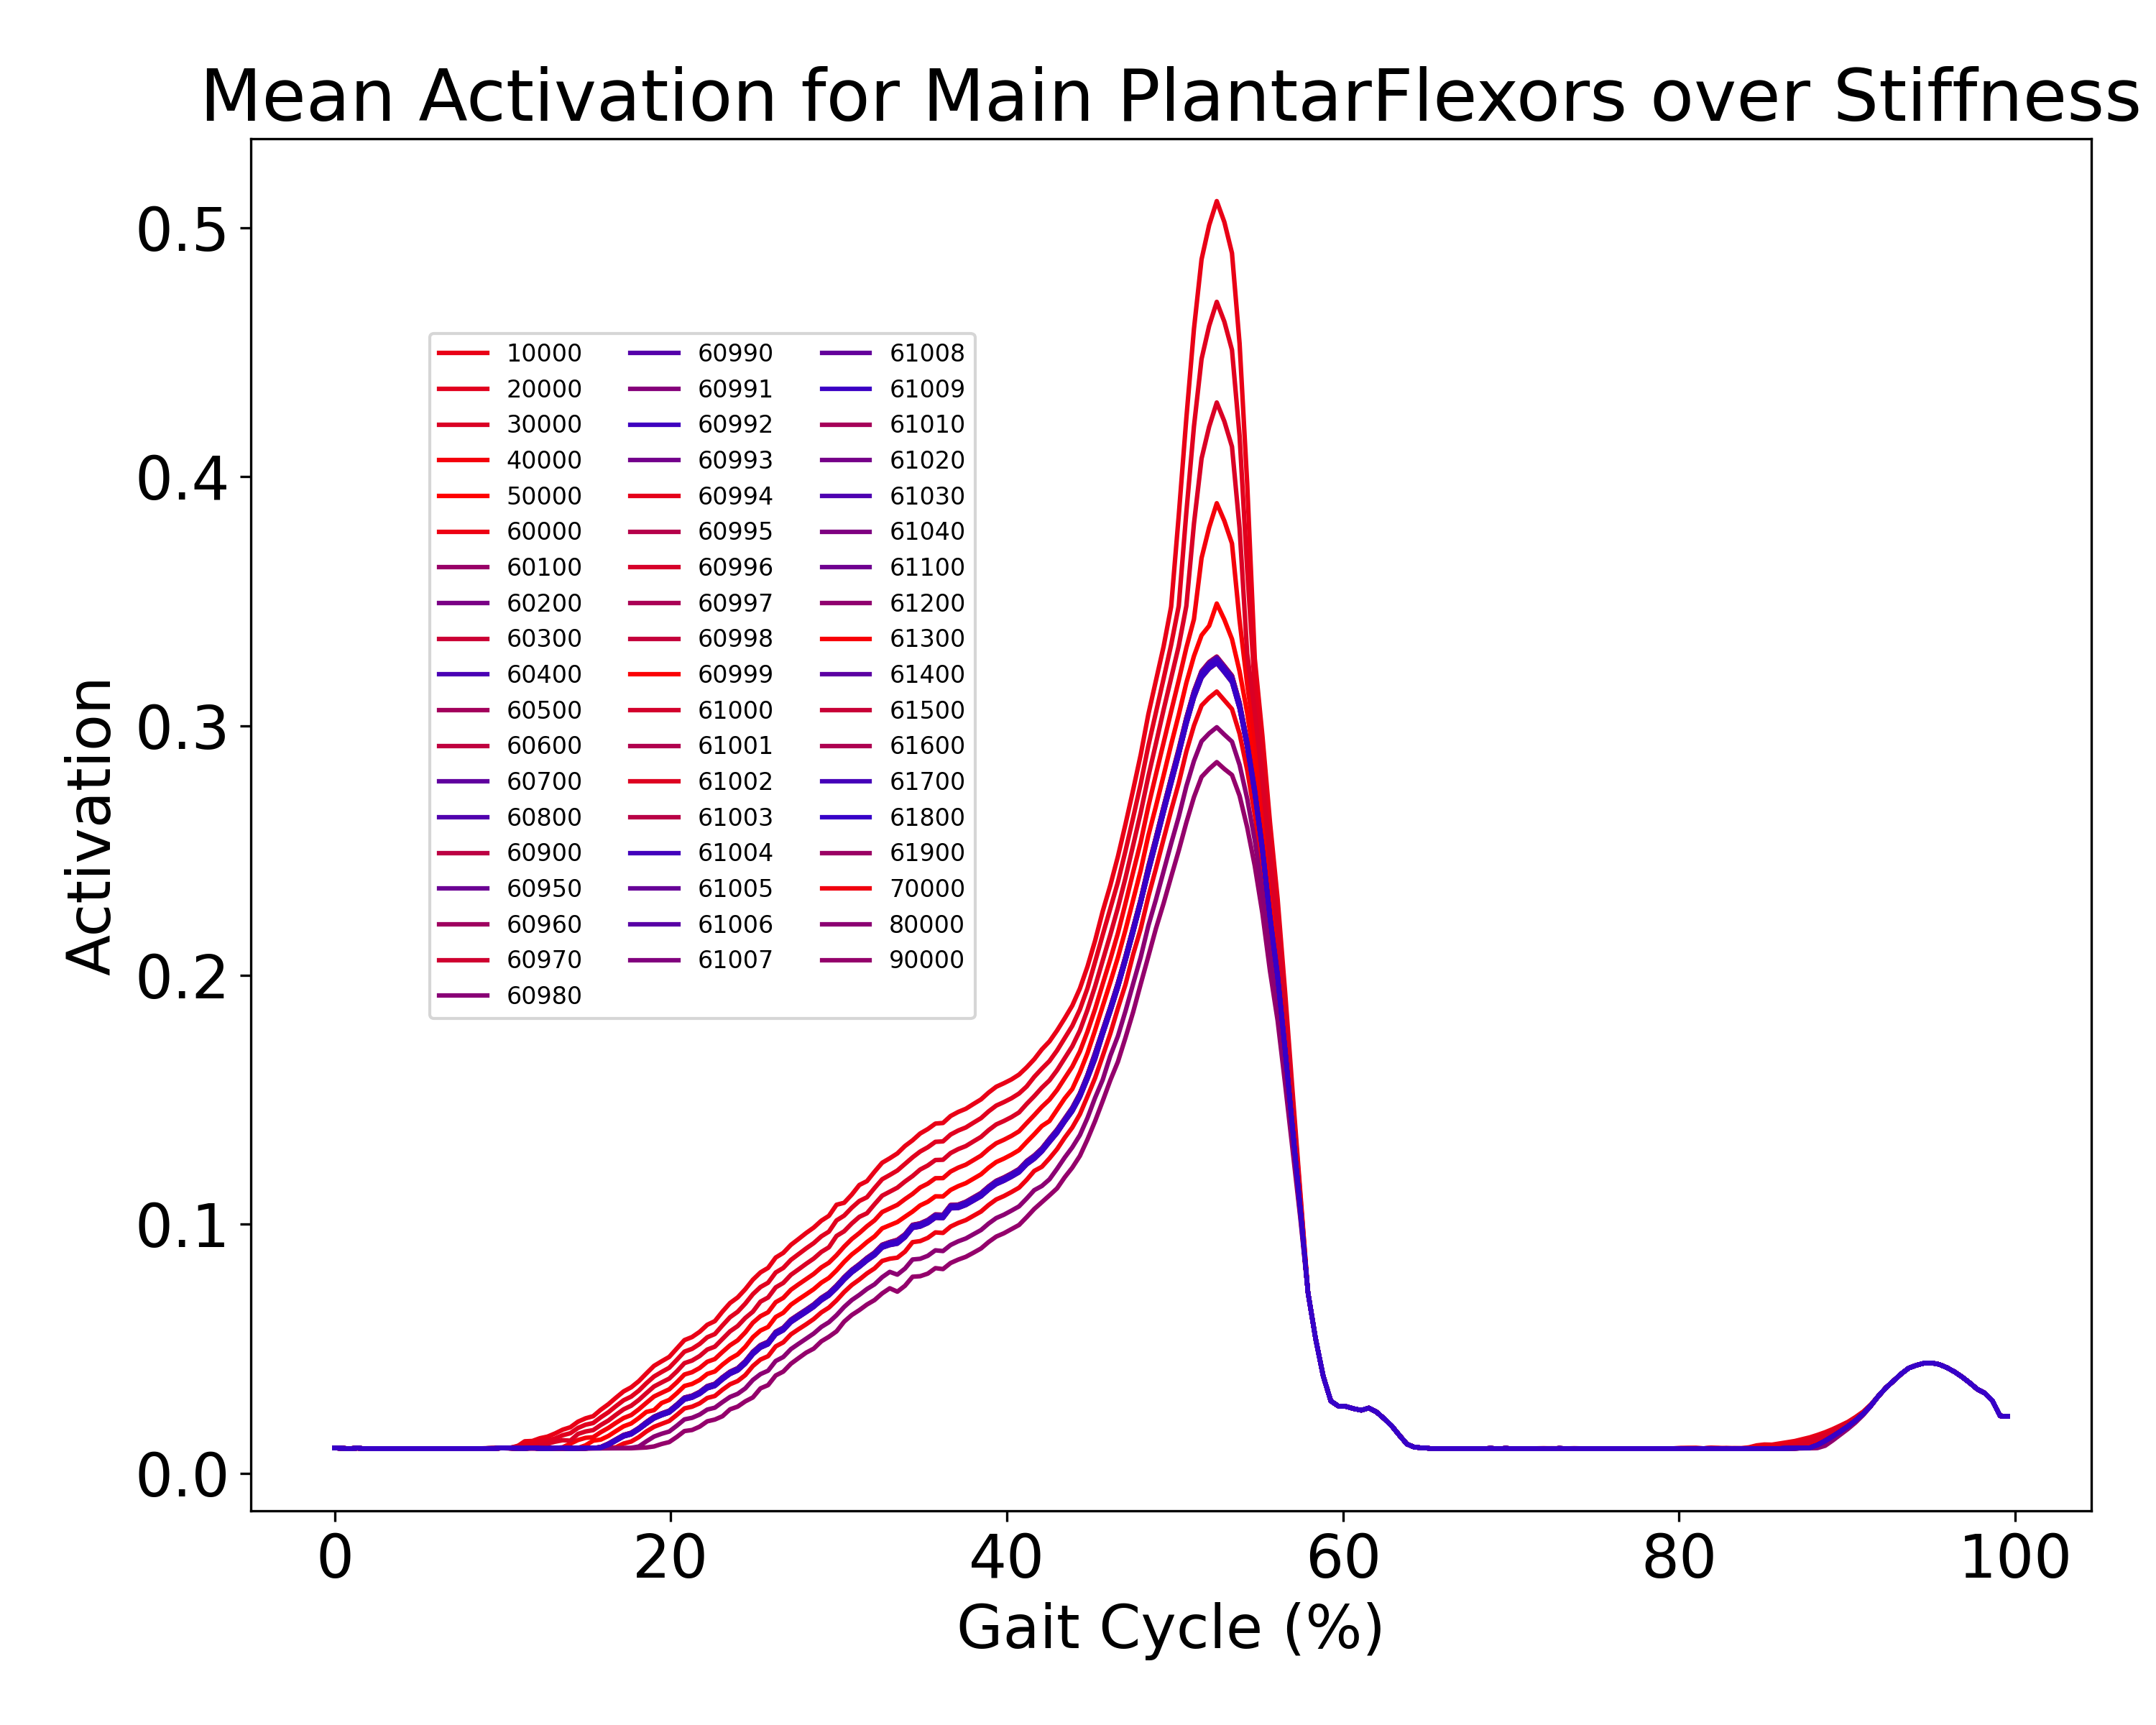
\includegraphics[width=\textwidth]{plots/stiffness/ActivationAcrossStiffness/TotalPlantarflexorsStiffness.png}
    \end{subfigure}
    \caption{Comparison of muscle activations for dorsiflexors and plantarflexors at different stiffnesses.}
\end{figure}

In the figure, we see how various muscles in the right foot are activated during the gait cycle. The muscles are divided into two groups based on their function:\\
\textbf{Dorsiflexors}: Tibialis Anterior, Extensor Digitorum, Extensor Hallucis, and Peroneus Tertius.\\
\textbf{Plantarflexors}: Tibialis Posterior, Gastrocnemius Medialis, Soleus, Peroneus Brevis, and Peroneus Longus.\\

\subsection*{Spring Power}

\begin{figure}[H]
    \centering
    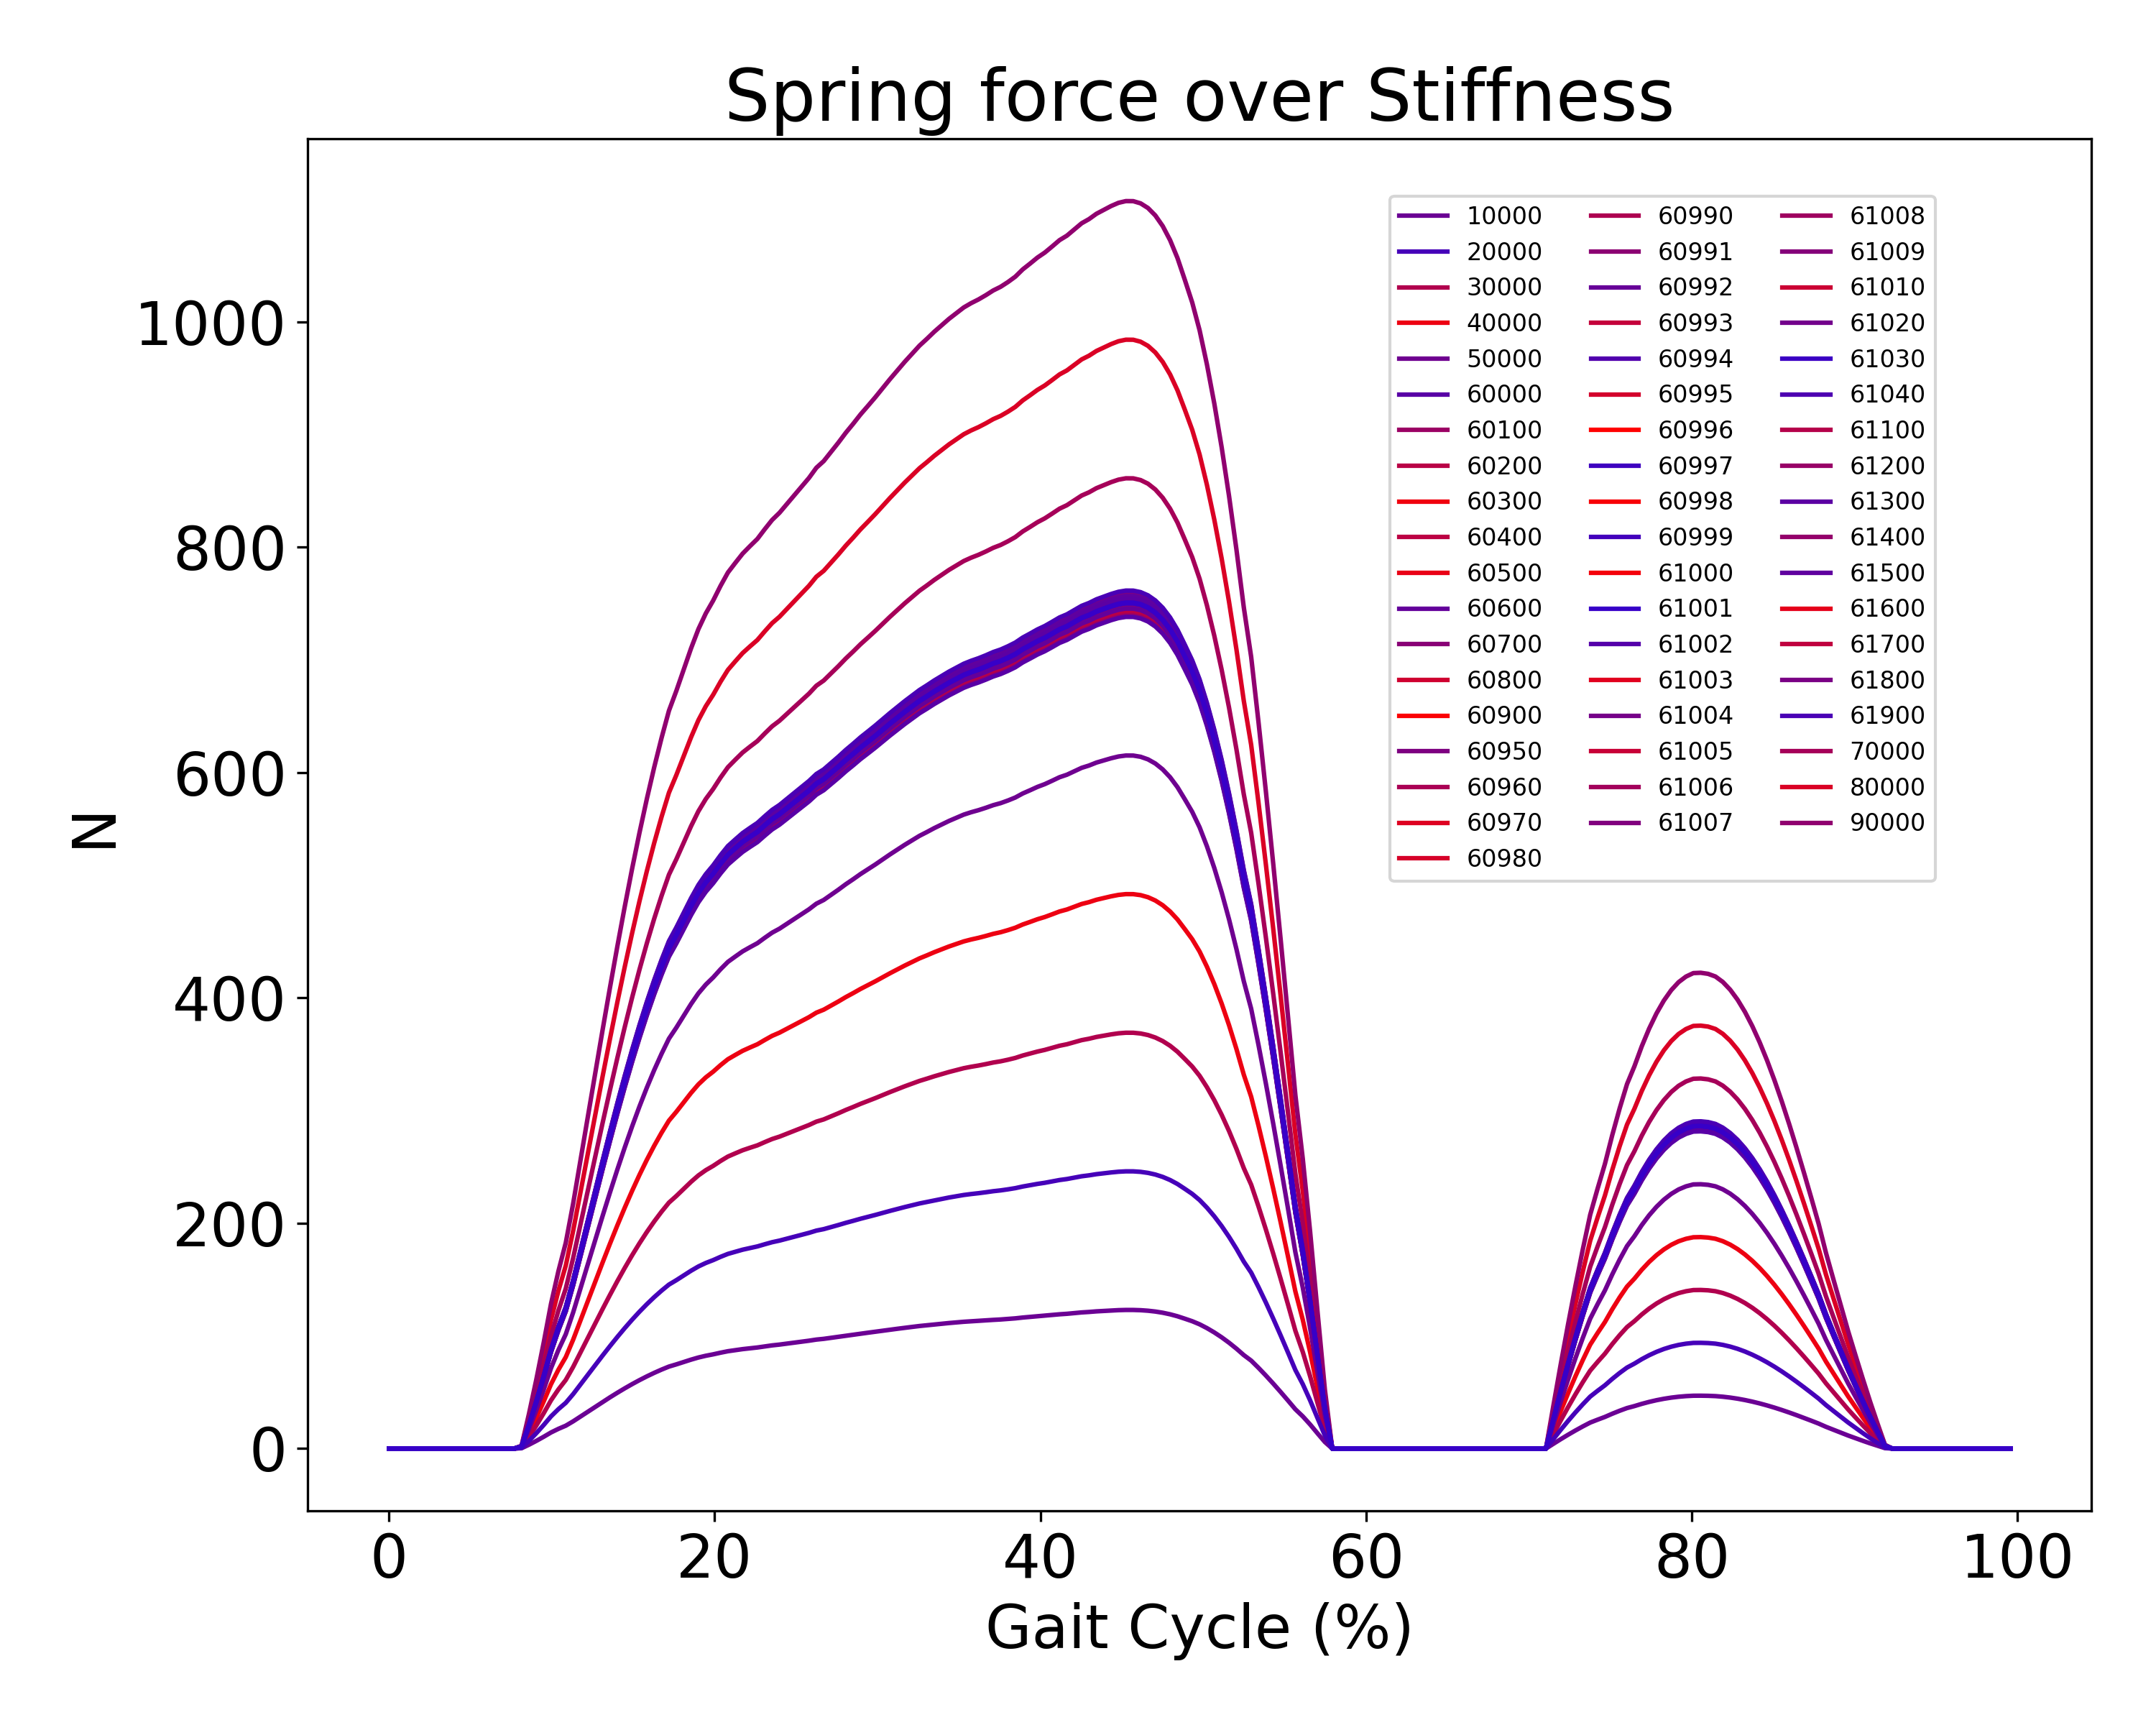
\includegraphics[width=0.6\textwidth]{plots/stiffness/ActivationAcrossStiffness/TotalSpringPowerStiff.png}
    \caption{Comparison of spring power over stiffness.}
\end{figure}

By looking at the stiffness graphs produced up to now, we see how increasing stiffness improves energy return but may simultaneously increase muscle activation demands, particularly for plantarflexors during push-off and dorsiflexors during swing clearance.

\section*{Resting Length}

\begin{figure}[H]
    \centering
    \begin{subfigure}[b]{0.42\textwidth}
        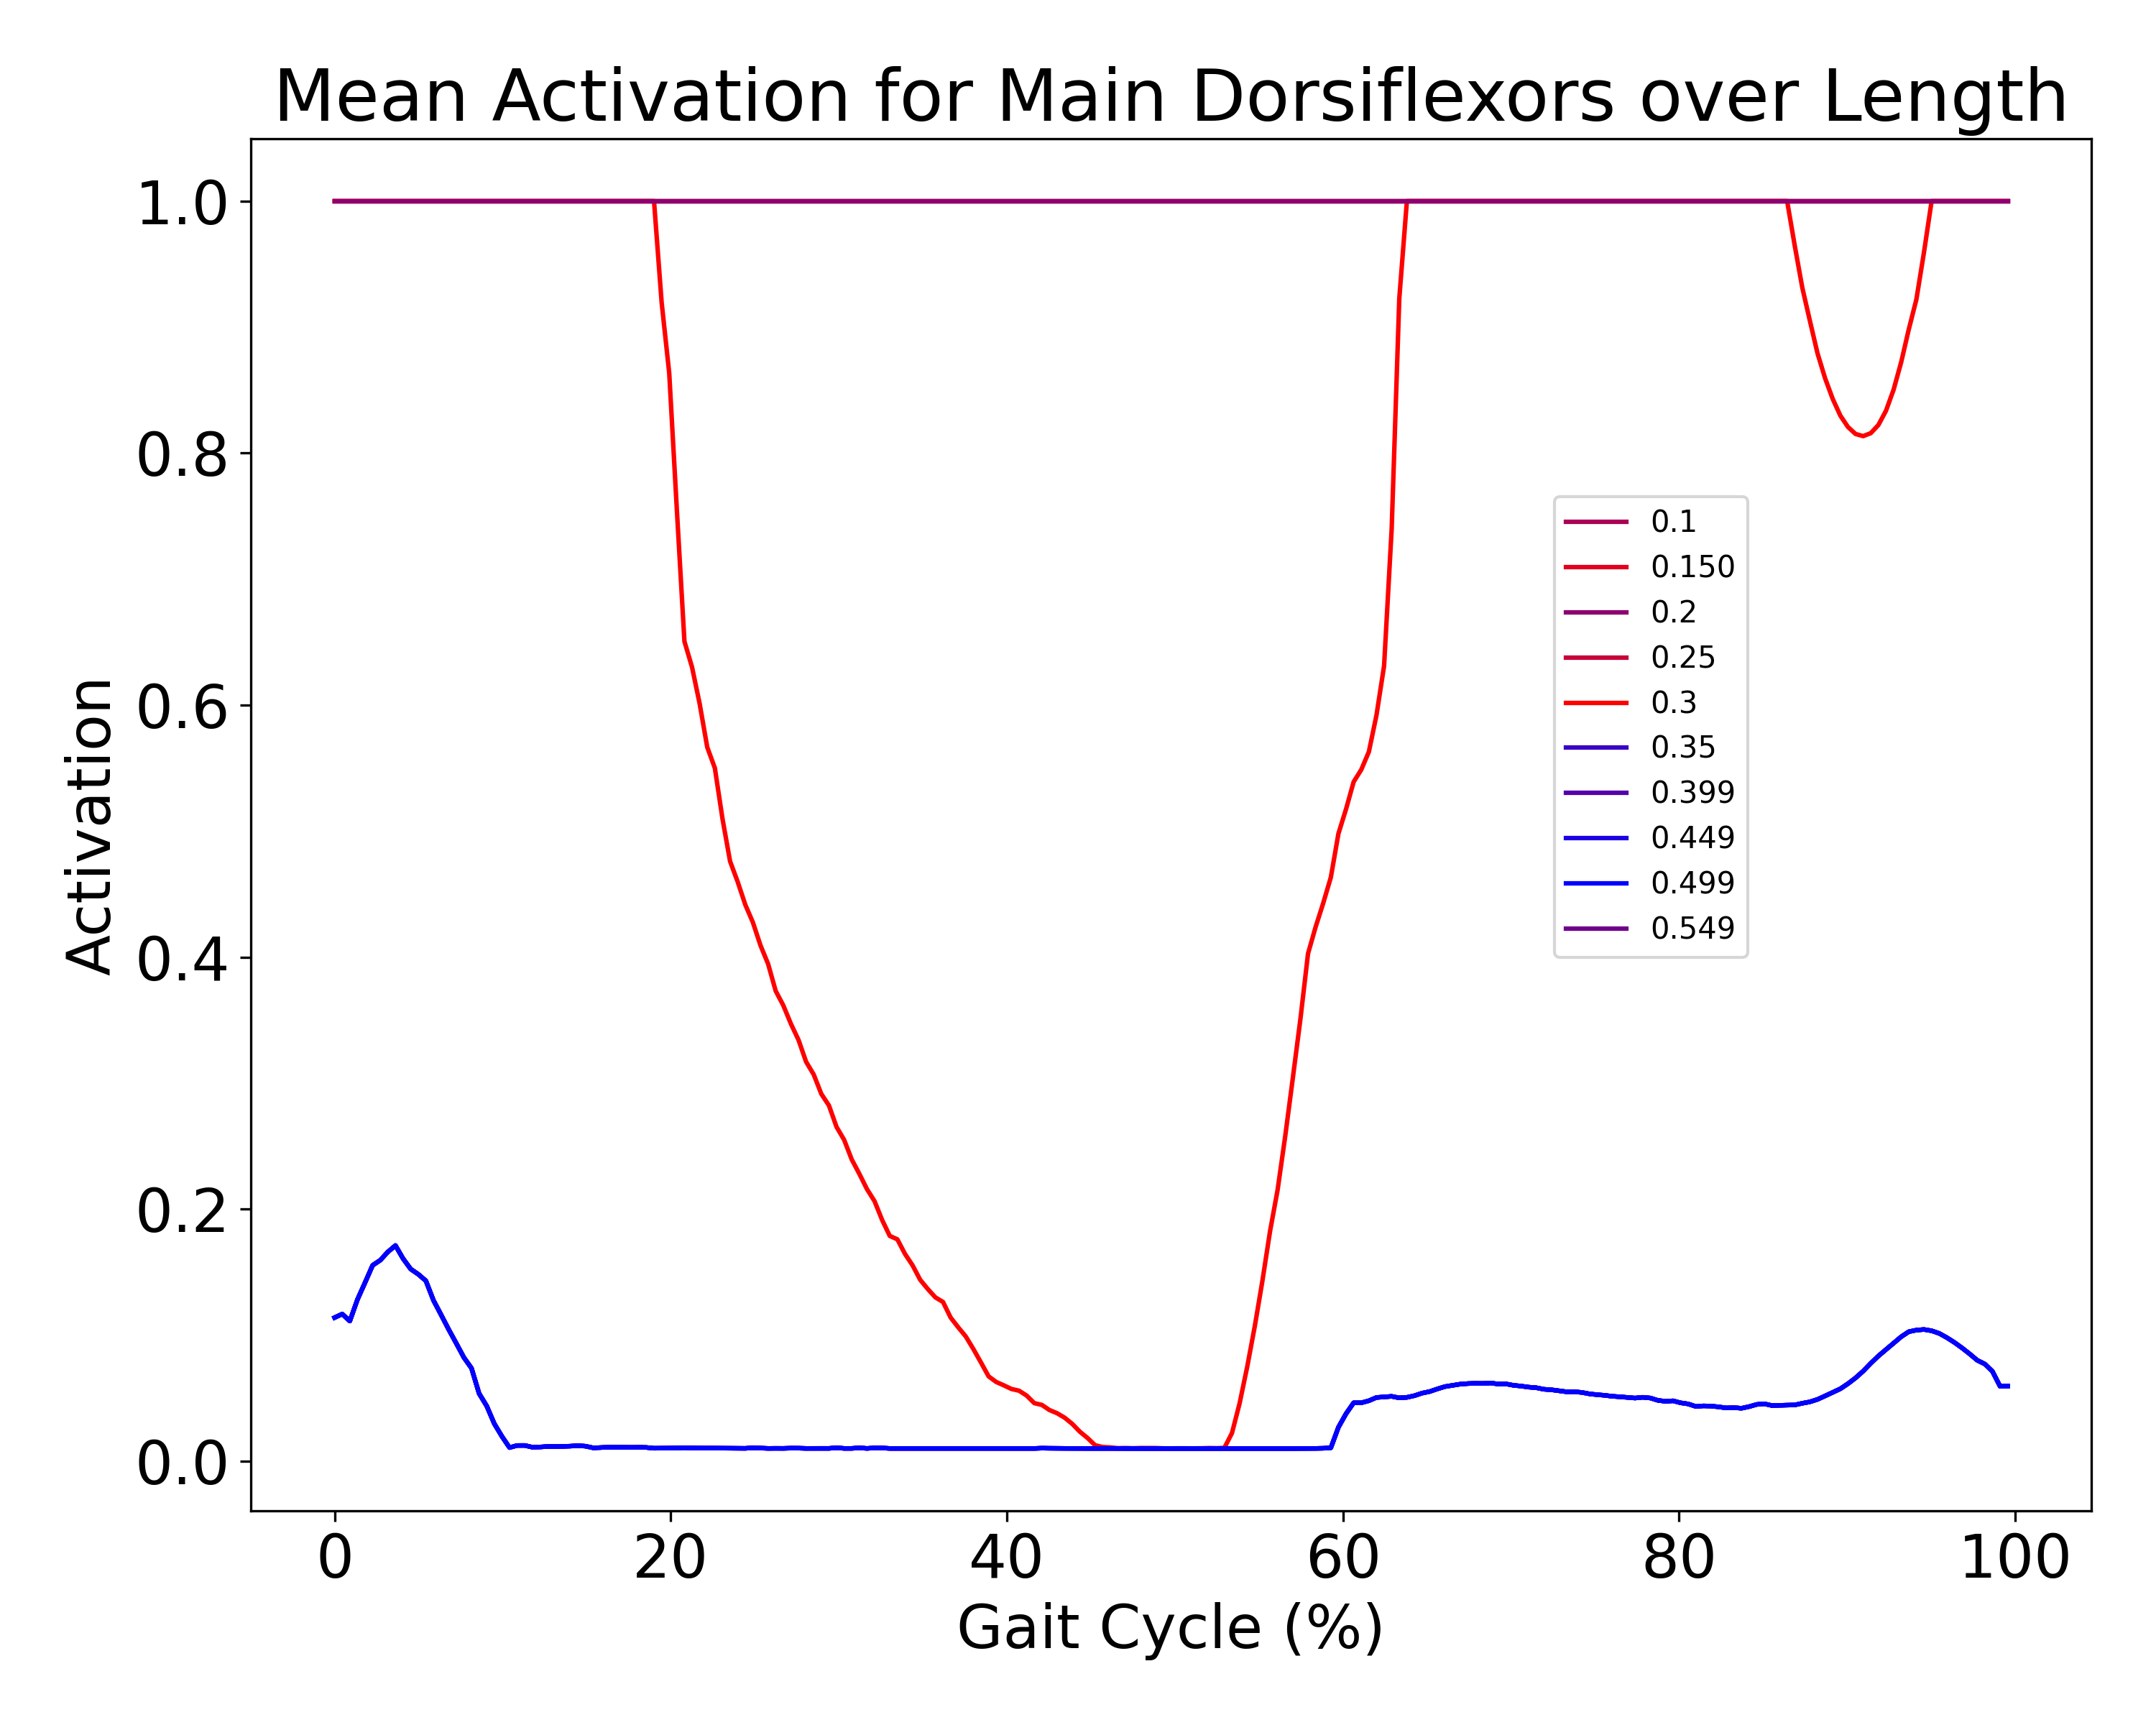
\includegraphics[width=\textwidth]{plots/restinglength/totalactivation/TotalDorsiflexorsLen.png}
    \end{subfigure}
    \hfill
    \begin{subfigure}[b]{0.42\textwidth}
        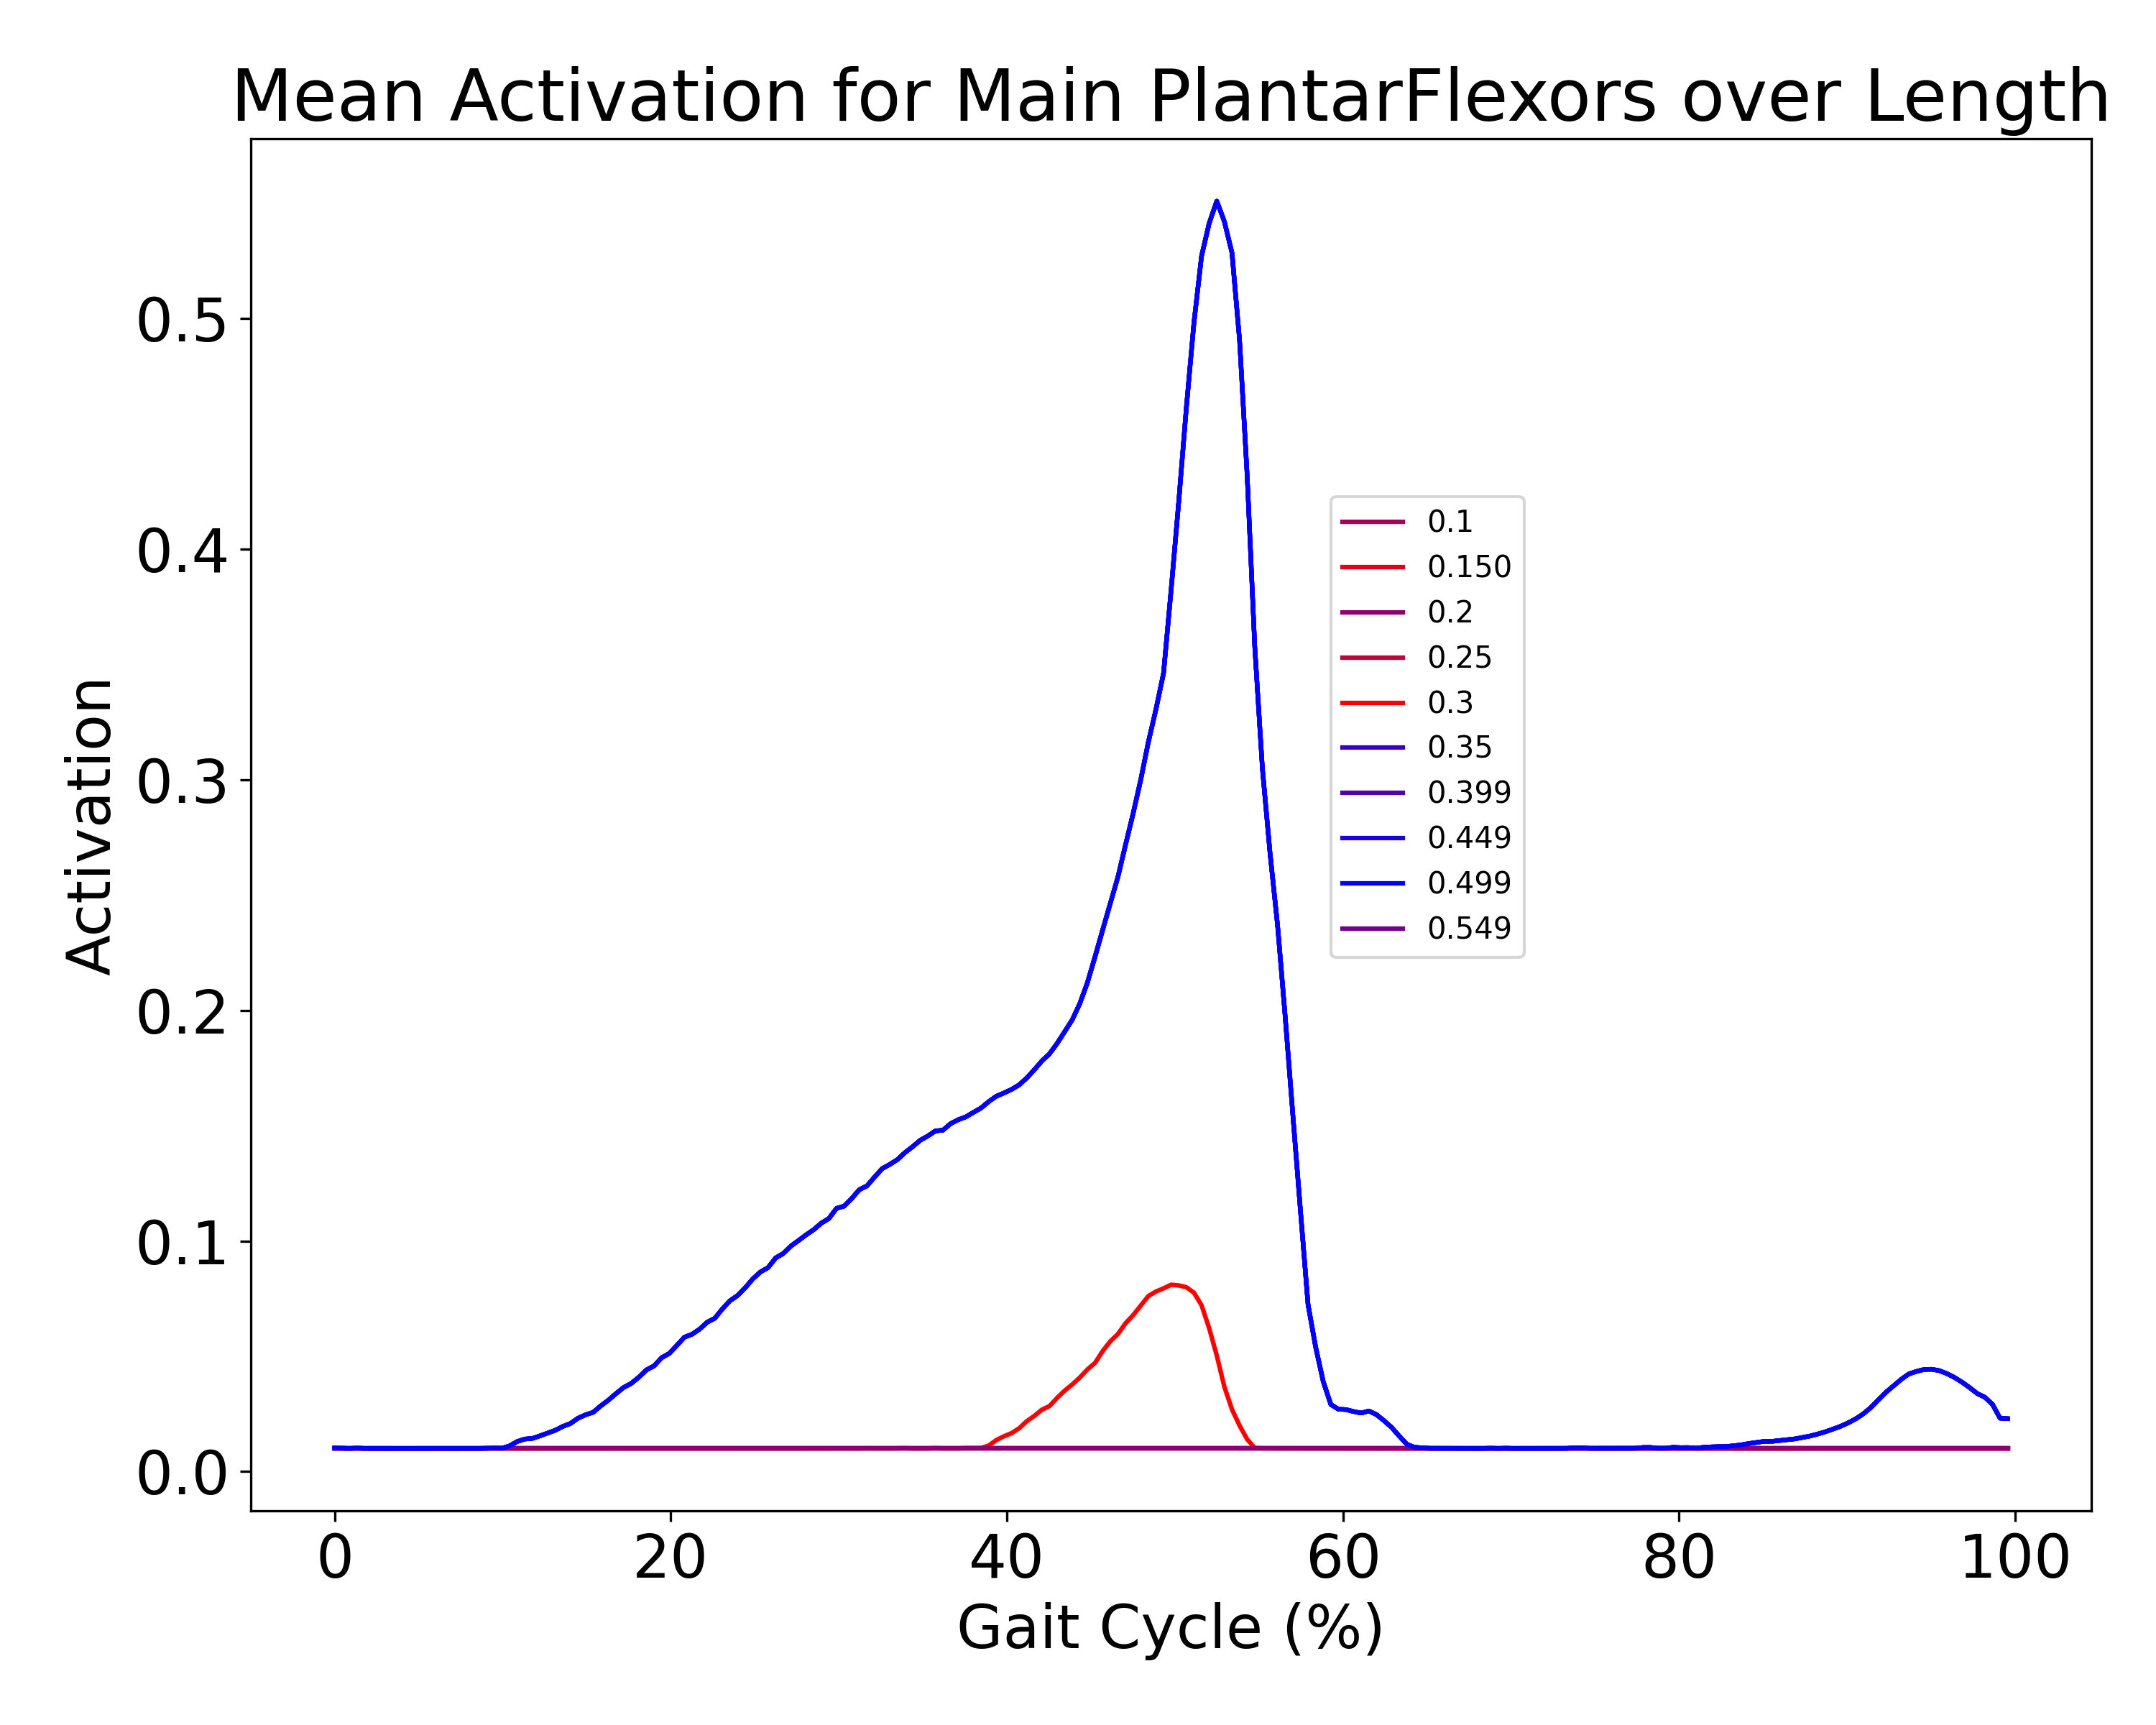
\includegraphics[width=\textwidth]{plots/restinglength/totalactivation/TotalPlantarflexorsLen.png}
    \end{subfigure}
    \caption{Comparison of mean activations for dorsiflexors and plantarflexors over resting length.}
\end{figure}

\section*{Design Proposal}

Optimal parameters: attachment distance 3cm, rest length  0.31m, stiffness 8000.0 N/m.

\end{document}
